\documentclass[11pt]{standalone}
\usepackage[usenames]{color} %used for font color
\usepackage{amssymb} %maths
\usepackage{amsmath} %maths
\usepackage[no-math]{fontspec}
\usepackage{unicode-math}
\usepackage{libertinus}
\usepackage{pgf,xcolor}
\definecolor{itwm_blue}{HTML}{005A94}
\definecolor{itwm_red}{HTML}{C00000}
\definecolor{itwm_yellow}{HTML}{e87846}
\definecolor{itwm_green}{HTML}{228B22}
\usepackage{tikz}
\usepackage{pgfplots}
\pgfplotsset{compat=newest}
\begin{document}
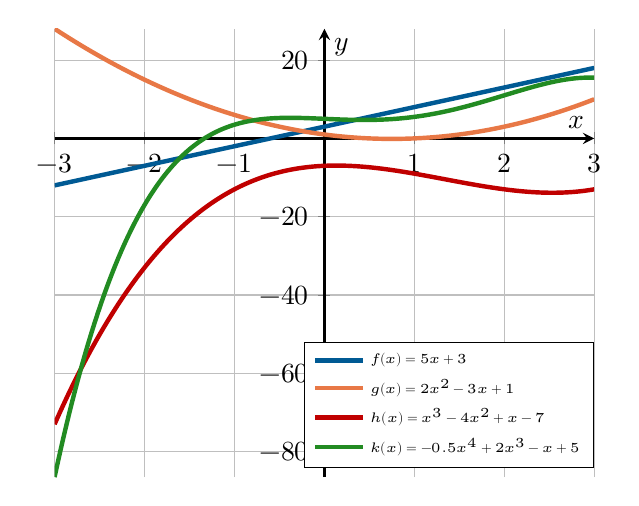
\begin{tikzpicture}
\begin{axis}[
    axis lines = center,
    xlabel = {$x$},
    ylabel = {$y$},
    xmin=-3.0, xmax=3.0,
    %ymin=-10.0, ymax=15.0,
    grid = both,
    axis line style={thick},
    legend style={font=\tiny, at={(1.0,0.02)}, anchor=south east},
    legend cell align=left,
    legend entries={$f(x) = 5x + 3$, $g(x) = 2x^2 - 3x + 1$, $h(x) = x^3 - 4x^2 + x - 7$, $k(x) = -0.5x^4 + 2x^3 - x + 5$},
]
    
\addplot[draw=itwm_blue, samples=300, ultra thick, domain=-3:3]{ 5*x + 3 };

\addplot[draw=itwm_yellow, samples=300, ultra thick, domain=-3:3]{ 2*x^2 - 3*x + 1 };

\addplot[draw=itwm_red, samples=300, ultra thick, domain=-3:3]{ x^3 - 4*x^2 + x - 7 };

\addplot[draw=itwm_green, samples=300, ultra thick, domain=-3:3]{ -0.5*x^4 + 2*x^3 - x + 5 };

\end{axis}
\end{tikzpicture}
\end{document}